\section{Tower: from Functions to Architectures}
\label{sec:tower}

In a typical embedded systems project, programmer must produce an entire
system of software that interacts with multiple input and output peripherals
concurrently using a real-time operating system (RTOS). Typical RTOSes provide
just a few low-level locking and signaling primitives for scheduling. Since
microcontrollers do not have virtual memory managment units (MMUs) found on
larger processors, the RTOS kernel can't protect the system against badly
behaved user code. These restrictions put significant burden on the programmer:
she must ensure all tasks and communication between tasks is implemented
correctly.

Luckily, we already have Ivory in our toolbox, which can provide lots of the
guarantees we need about task memory safety. To handle the rest of these
concerns, we have built Tower, an EDSL for specifying tasks and communication
channels that generates correct Ivory implementations, as well as architecture
description artifacts.

Tower's code generation approach offers safety guarantees because it does not
expose the dangerous low-level scheduling primitives to the user, and it keeps
type information for channels (i.e. the datatype of the channel message),
expressed as Ivory types, in the Haskell type system.

Tower allows the programmer to describe a static graph of channels and tasks.
This is a restriction of the capabilties of most operating systems, which may
create and destroy tasks or communication datastructures at run-time. However,
for the intended use case in high assurance systems, a static configuration of
channels and tasks makes it easier to reason about memory requirements, and
permits the system to be analyzed for schedulability.

The static tower graph of channels and tasks also makes it possible to
describe the system architecture to external tools. Tower has a backend which
generates a system description in the Architecture Analysis and Design Language
(AADL)\ph{cite}. Other backends, such as for the Graphviz dot language, exist as well.
These output formats make it possible to visualize, analyze, and automatically
check properties about the system, without knowing anything about Haskell,
Ivory, or Tower. This is an important feature when working with teams that may
not all be literate in Ivory/Tower.

%% The user specifies Tower tasks and channels with a Haskell embedded DSL. The
%% Tower library presents a monadic interface for creating tasks and channels.
%% This makes it natural to use the full power of the host language as a macro
%% system for Tower. The user can specify their Haskell functions, types, and
%% modules for building system components using Tower. This permits the user to
%% build higher level abstractions than Tower provides, and use Haskell semantics
%% to get improved safety assurances about their code.

Tower structures tasks as an event loops,  with a callback specified in Ivory to
handle each  event. Tower  tasks traditionally register  channels and  timers as
event sources\ph{what's source here?}. Tower  also has a facility for registering  callbacks on external
events, which, with  some help from a platform-specific backend,  can be used to
handle hardware  interrupts. Combined  with Ivory  extensions for  safe hardware
register manipluation, we have  implemented several low-level peripheral drivers
for the STM32F4 microcontroller in Tower.  \ph{this para is a little dense.}

Since Tower has a complete description of both the task glue code and Ivory
implementation, a top level description of a system can be used directly to
generate all of the C code for a microsystem system image.

Tower is designed to support different operating systems via a swappable
backend. Since all code that touches operating system primitives is generated by
Tower, it is trivial for the user to specify a system and compile it for
different operating systems. Tower supports both the open-soure
FreeRTOS\footnote{\url{http://www.freertos.org/}} as well as the
formally-verified eChronos
RTOS\footnote{\url{http://ssrg.nicta.com.au/projects/TS/echronos/}} development
by NICTA.

\begin{figure}
  \begin{center}
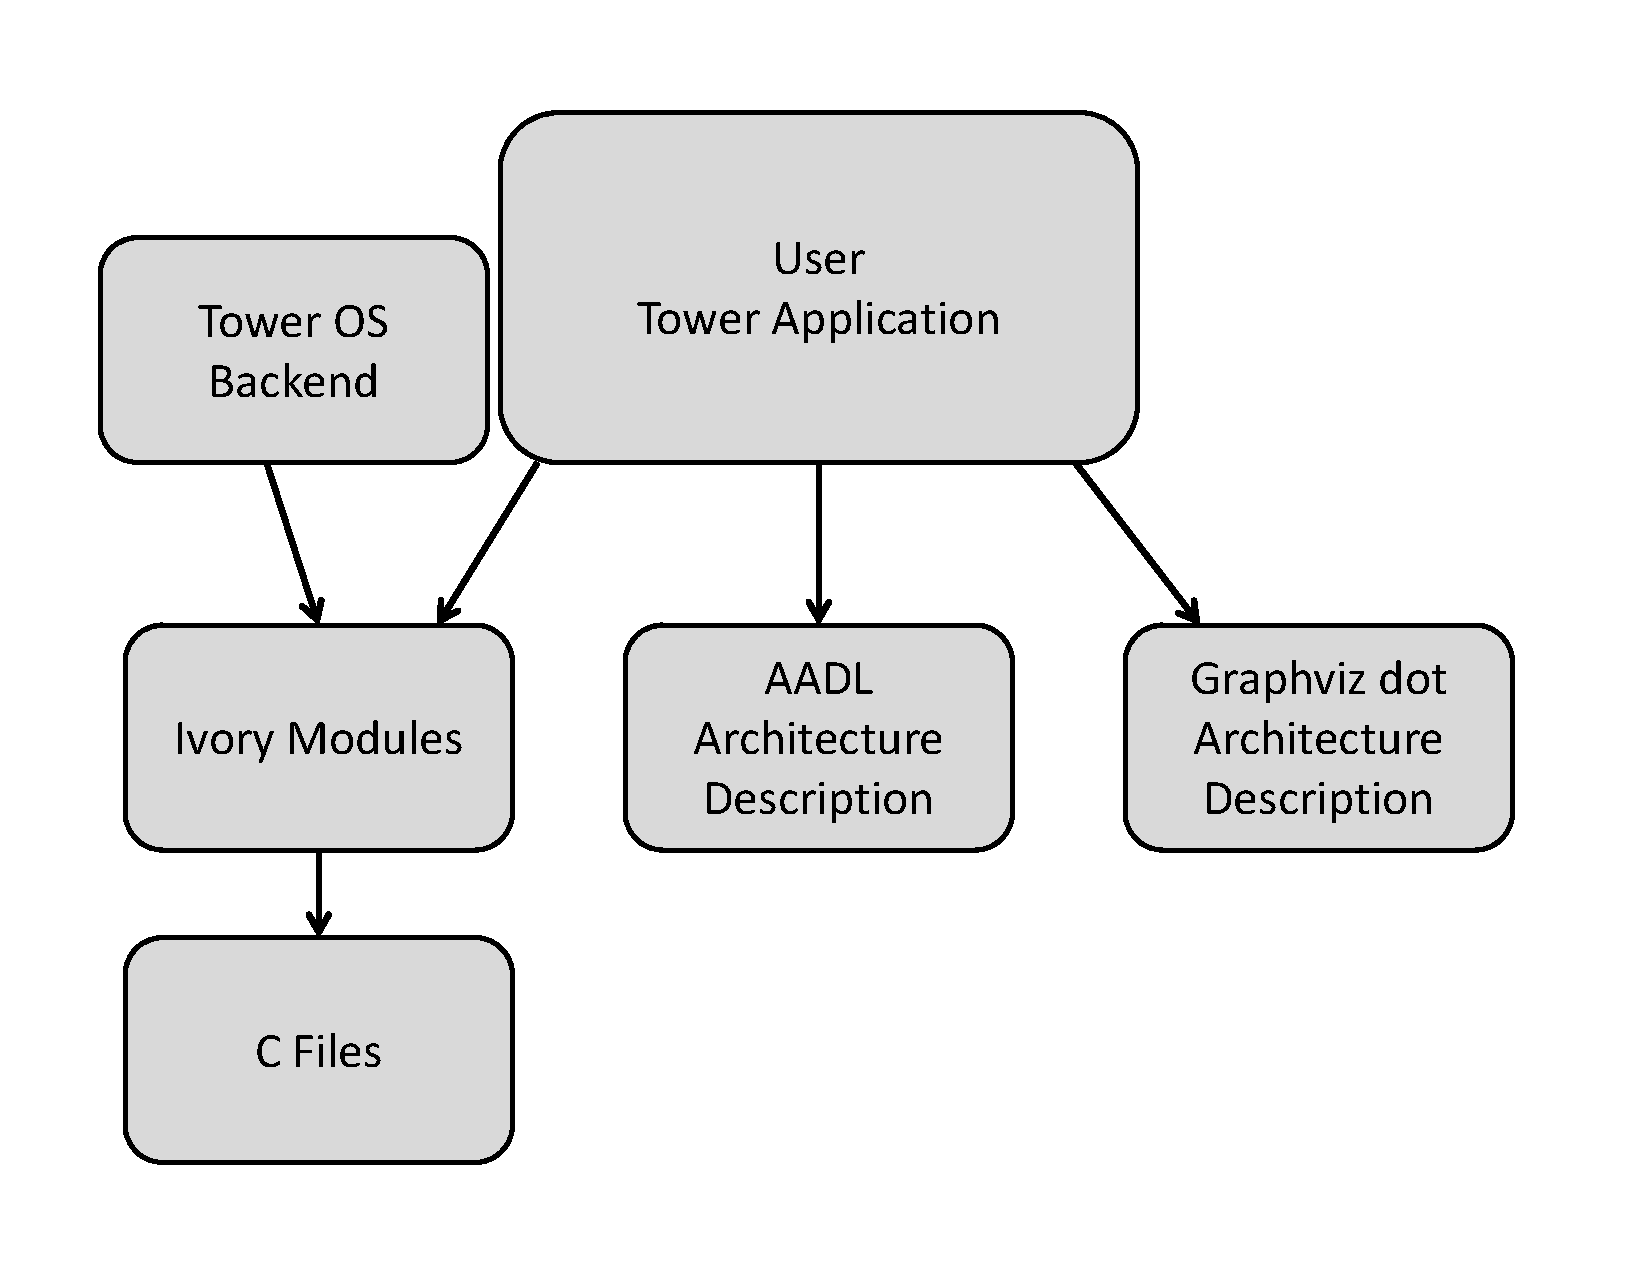
\includegraphics[width=6cm]{figures/tower-artifacts-dia}
  \end{center}
  \caption[Tower artifacts]{Tower artifact generation.}
\label{fig:towerArtifacts}
\end{figure}
\ph{can you move the c-files box to the side so less vertical room is taken up?}

\ph{you don't reference the tower figure?}
\ph{Give a tower example---maybe the LED driver example from the talks.}
\ph{Show a diagram showing what all Tower generates---that'll help the text.}
